\documentclass[11pt]{article}

\usepackage{../algebra}

\begin{document}

\coverpage{8}

% hw problem 1 -----------------------------------------------------------------

\begin{exercise}{87}{2}
    \problem{
        Let $G$ be the group of all real-valued functions on the unit interval $[0,1]$, where we define, for $f, g \in G$, addition by $(f+g)(x) = f(x) + g(x)$ for every $x \in [0,1]$.
        If $N = \{ f \in G \mid f(1/4) = 0 \}$, prove that $G/N \cong $ the real numbers under $+$.
    }
    \proof{
        Note that our ambient group $G$ is abelian so any subgroup is a normal subgroup.
        We first claim that $N \leq G$ by showin the aesthetic definition holds for $N$.
        Certainly $id \in N$ for $id (1/4) = 0$.
        Now pick $f,g \in N$ and recall that $g^{-1} = - g$.
        Then $f + g^{-1} = f + (-g)$ and now evaluating at $x=1/4$: $(f+(-g))(1/4) = f(1/4) + (-g(1/4)) = 0 + -0 = 0$ so $f + g^{-1} \in N$. \parspace
        Now the quotient group $G / N = \{ g + N \mid g \in G \}$ and $(g+N)(1/4) = g(1/4) + N(1/4) = g(1/4) + 0 = g(1/4)$.
        Let's define the mapping $\psi: G/N \to \R$ which takes $g + N$ to $g(1/4)$.
        We must verify four things for $\psi$ to be an isomorphism: well-defined, homomorphism, onto, and 1-1. \parspace
        Well-defined: pick $g + N = \bar g + N$.
        Then there exists some $f \in N$ such that $g = \bar g + f$ which implies that $\bar g = g + f$.
        Now consider $\psi (\bar g + N) = \psi (g + f + N) = (g + f)(1/4) = g(1/4) + f(1/4) = g(1/4) = \psi (g + N)$ where we know $f(1/4) = 0$ since $f \in N$. \parspace
        Homomorphism: fix $g_1 +N, g_2 + N \in G / N$.
        Certainly we have $\psi (g_1 + N) + \psi (g_2 + N) = g_1(1/4) + g_2 (1/4)$.
        But we also have $\psi (g_1 + N + g_2 + N) = \psi (g_1 + g_2 + N) = (g_1 + g_2)(1/4) = g_1 (1/4) + g_2 (1/4) $ so $\psi$ is a homomorphism. \parspace
        Onto: this is verified quite easily.
        If you give me an $x^\star \in \R$, I will give you the function $f(x) = x^\star$ for $x \in [0,1]$.
        Certainly $\psi (f + N) = f(1/4) = x^\star$. \parspace
        1-1: fix any $f_1, f_2 \in G$ such that $\psi (f_1 + N) = \psi (f_2 + N)$.
        We wish to show that $f_1 + N = f_2 + N$ which is true if there exists some $n \in N$ such that $f_1 = f_2 + n$.
        We will provide such a function $n(x)$.
        Note that $\psi (f_1 + N) = \psi (f_2 + N) \implies f_1 (1/4) = f_2 (1/4)$.
        Here is our function defined on $[0,1]$:
        \[ n(x) =
        \begin{cases}
            0 & x = 1/4 \\
            f_1(x)-f_2(x) & x \neq 1/4
        \end{cases}
        \]
        Now consider $f_2(x) + n(x)$.
        If $x = 1/4$ then $f_2(1/4) + n(1/4) = f_2 (1/4) + 0 = f_1 (1/4)$.
        Then if $x \neq 1/4$ we have $f_2 (x) + n(x) = f_2 (x) + f_1 (x) - f_2 (x) = f_1 (x)$.
        Thus $f_1 (x) = f_2 (x) + n(x)$ for all $x \in [0,1]$ and we have $f_1 = f_2 + n$ which implies that the cosets $f_1 + N$ and $f_2 + N$ are equal.
        Thus $\psi$ is 1-1. \parspace
        We have check everything we need to for $\psi$ to be an isomorphism so the two groups are isomorphic!
    }
\end{exercise}

% hw problem 2 -----------------------------------------------------------------

\newpage
\section*{3rd Iso Thm Example}
    \problem{
        Identify and illustrate with pictures the three quotient groups in the 3rd isomorphism theorem instantiated for $G = \R \times \Z _2$, $N = \Z \times \Z _2$, and $K = 2\Z \times \{ 0 \}$.
    }
    \proof{
        For this problem and the next, I ended up drawing a lot of pictures so all my work is in the figures below.
        \begin{figure}[h]
            \centering
            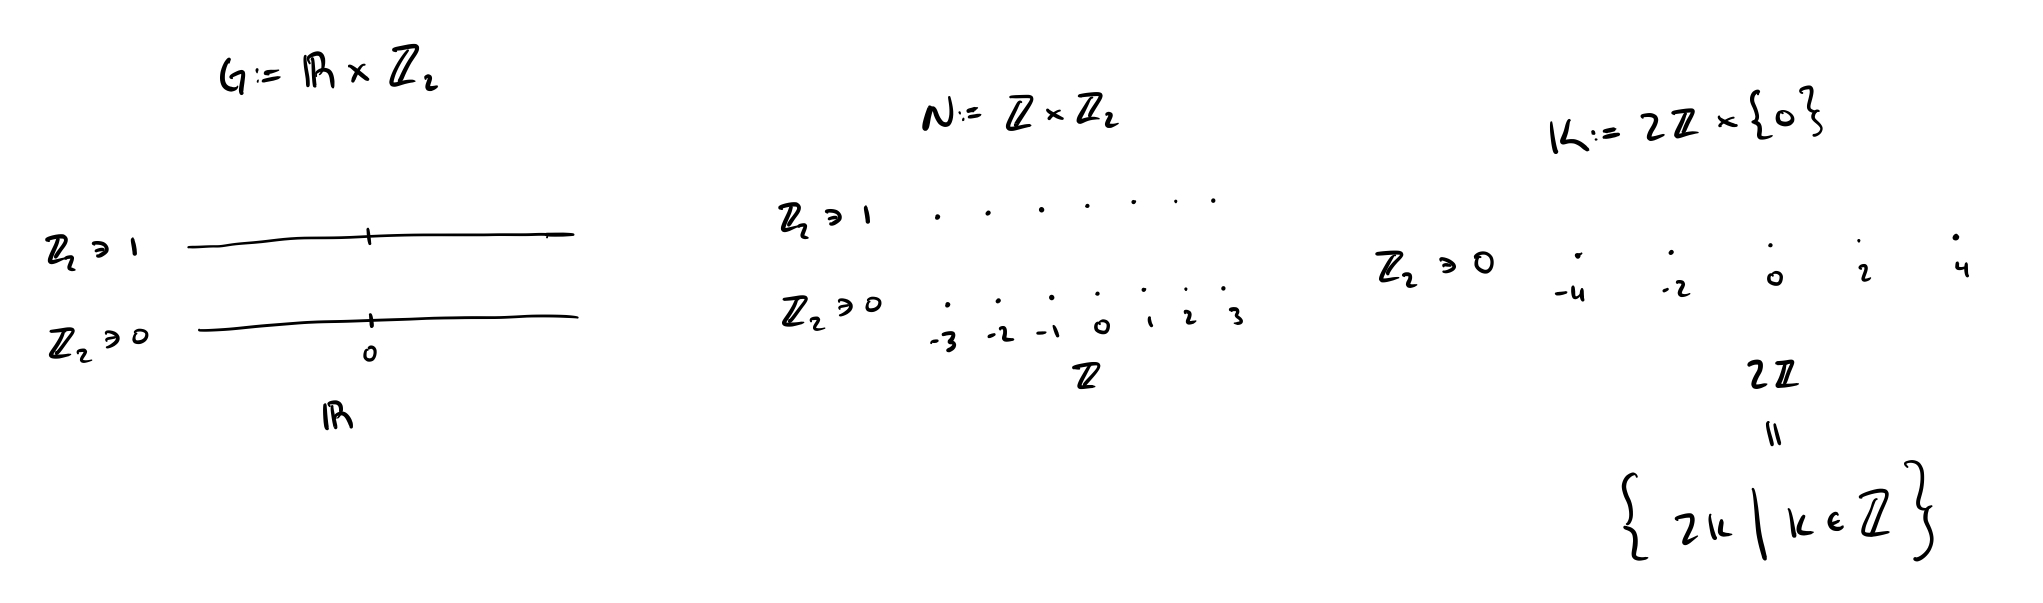
\includegraphics[width=0.95\textwidth]{images/3isothminit}
            \label{fig:3isothminit}
        \end{figure}
        \begin{figure}[h]
            \centering
            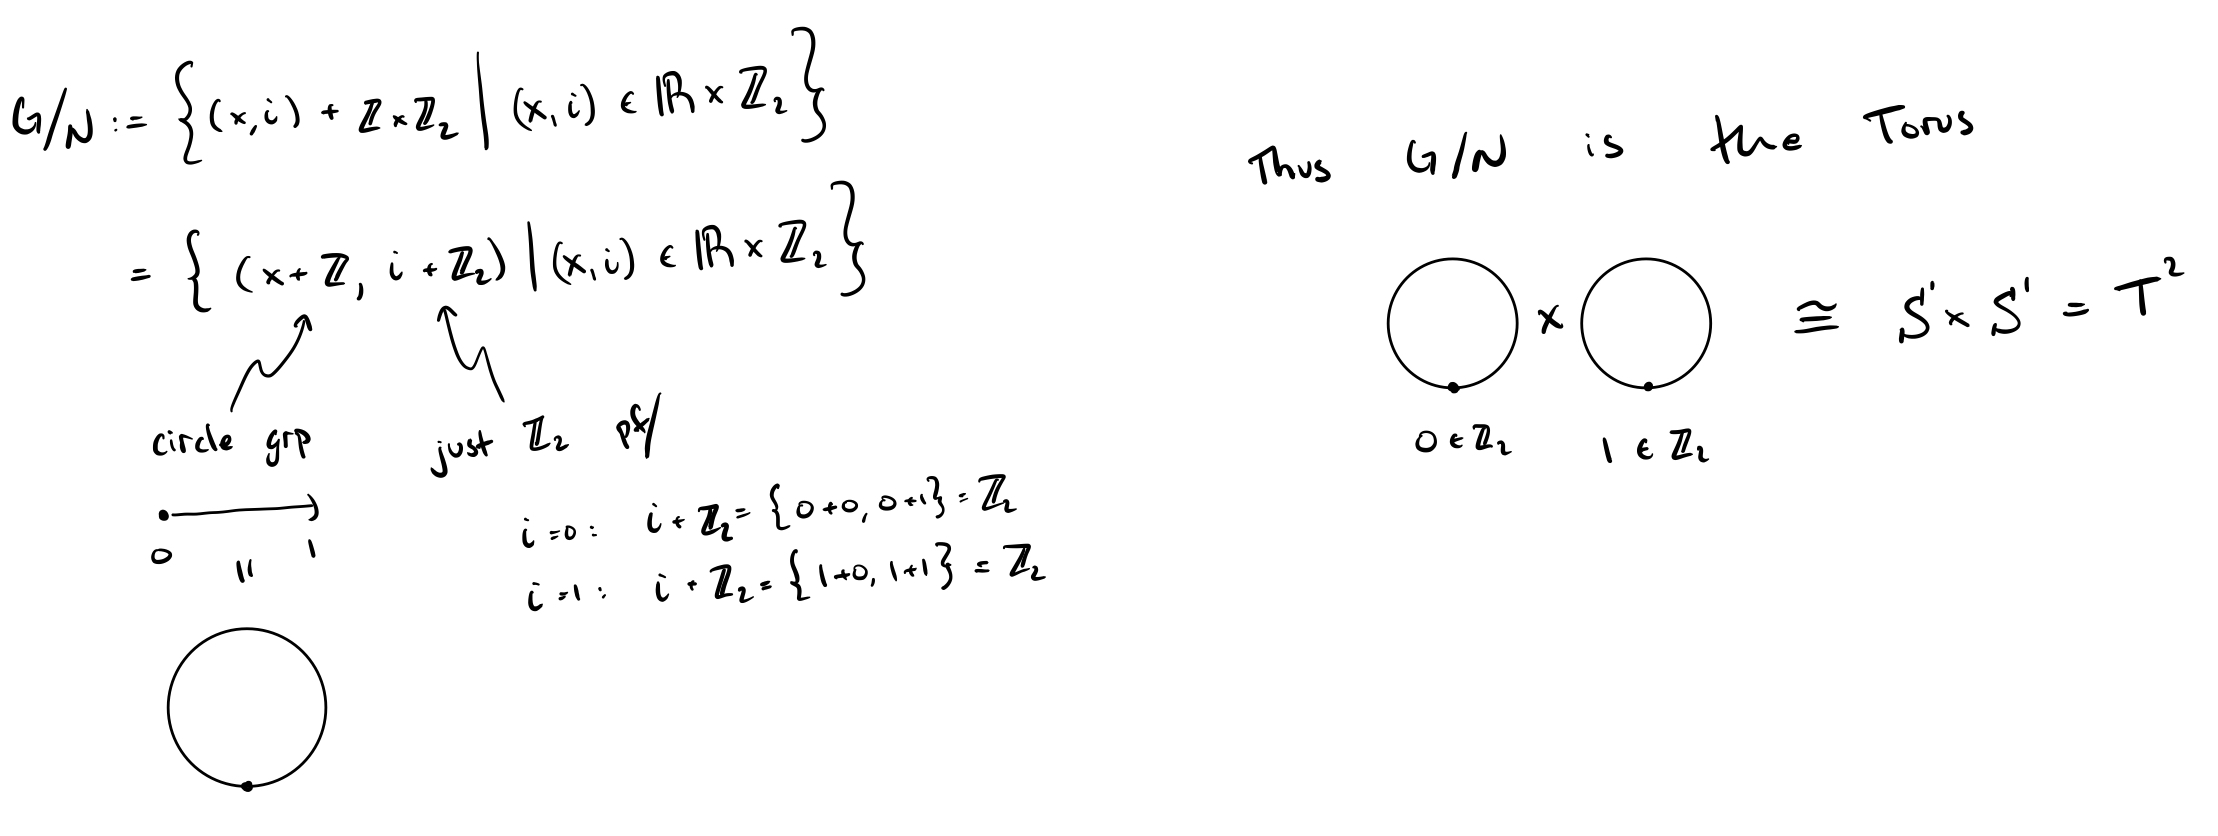
\includegraphics[width=0.95\textwidth]{images/GmodN}
            \label{fig:GmodN}
        \end{figure}
        \begin{figure}[h]
            \centering
            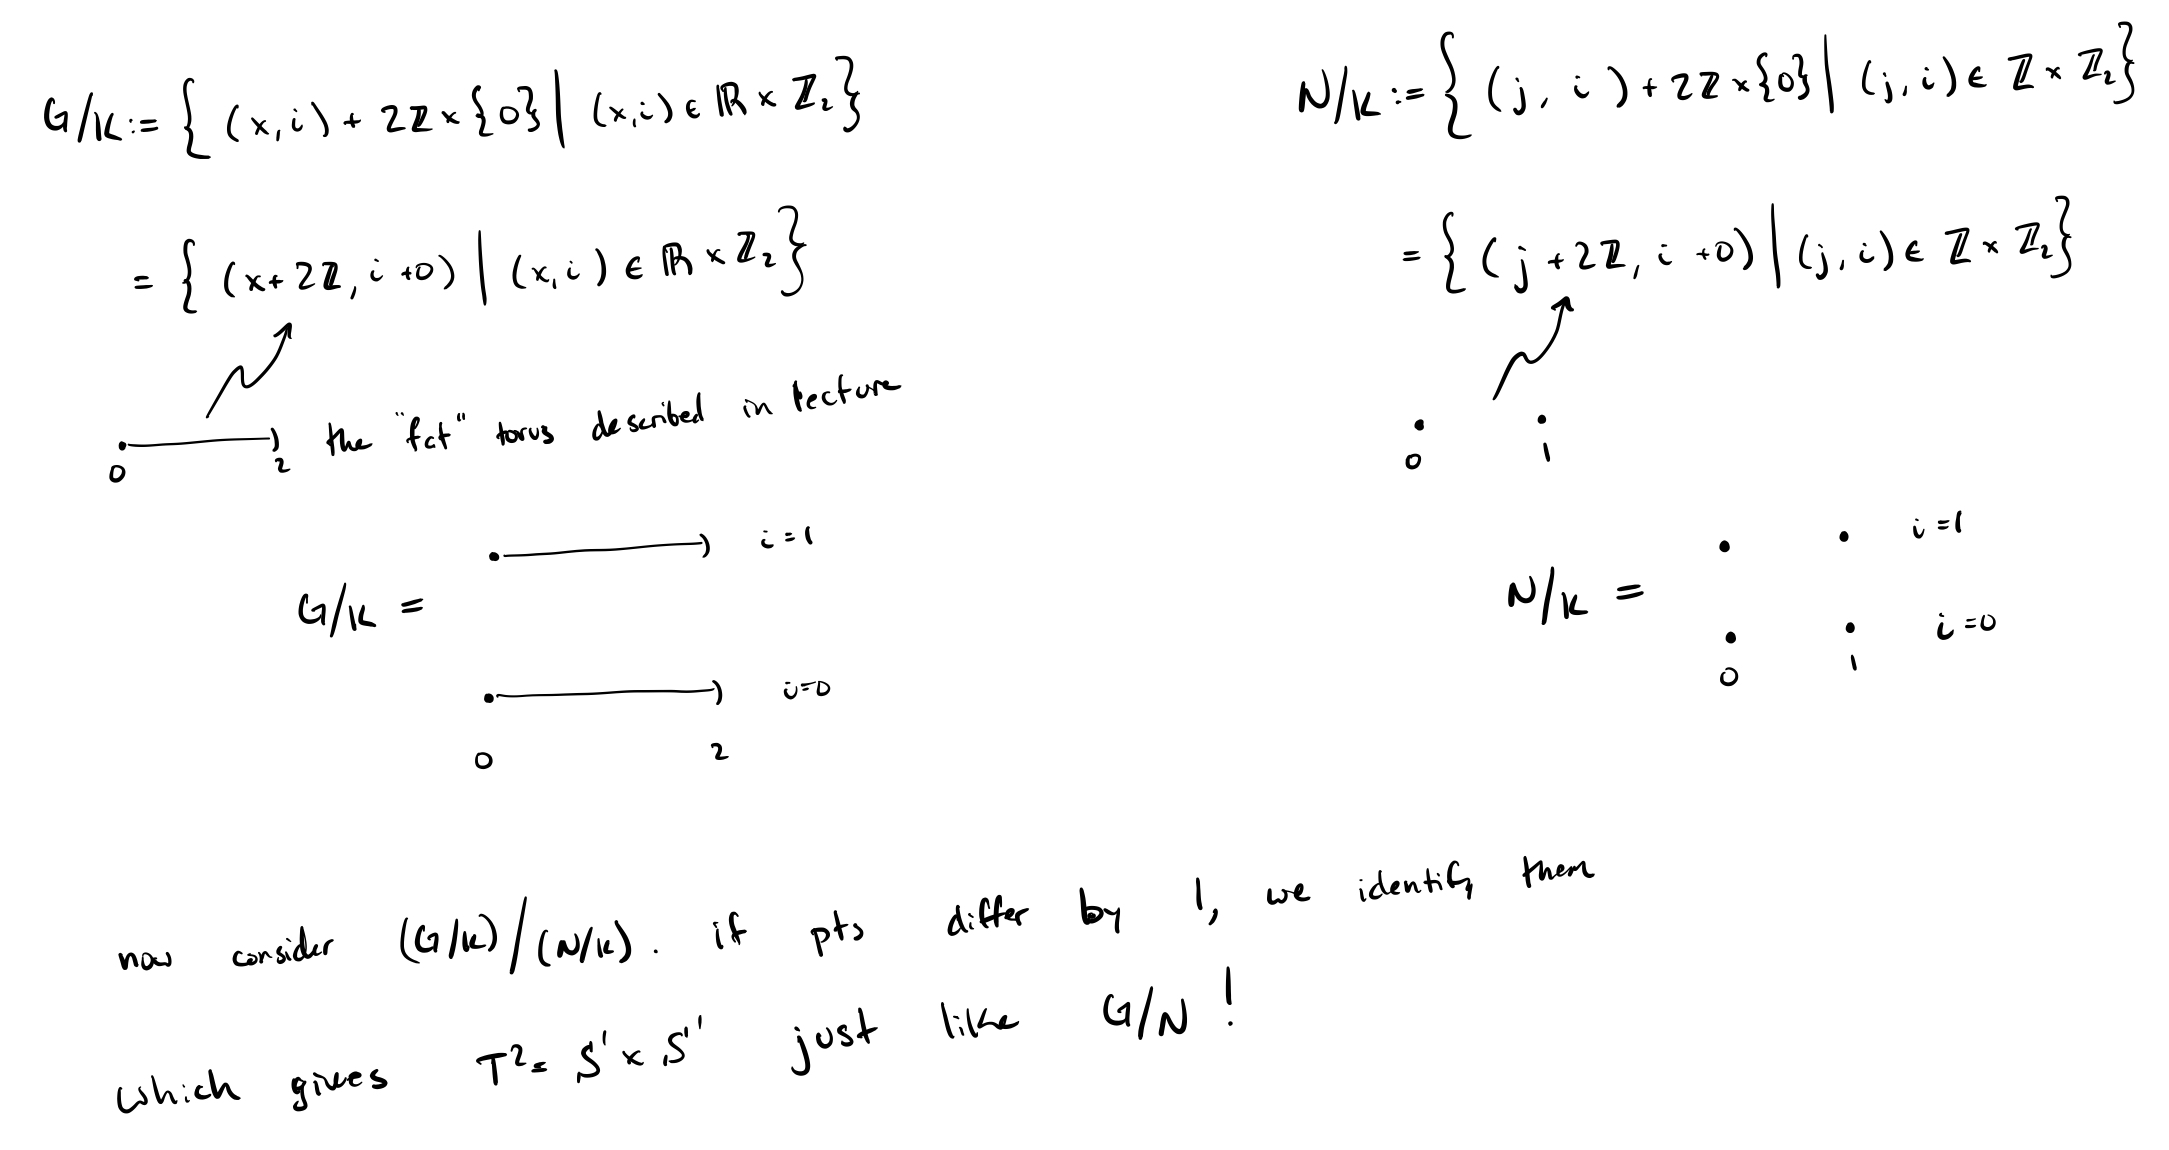
\includegraphics[width=0.95\textwidth]{images/GmodKNmodK}
            \label{fig:GmodKNmodK}
        \end{figure}
        \newpage
        Thus we have depicted the groups!
    }


% hw problem 3 -----------------------------------------------------------------

\newpage
\section*{2rd Iso Thm Example}
    \problem{
        Identify and illustrate with pictures all the groups involved in the 2nd isomorhpism theorem isntantiated for $G = \R \times \R$, $N = \Z \times \R$, $H = \R \times \{ 0 \}$.
        In particular, draw the cosets making up the quotient groups and recognize the groups as familiar concrete groups.
    }
    \proof{
        \begin{figure}[h]
            \centering
            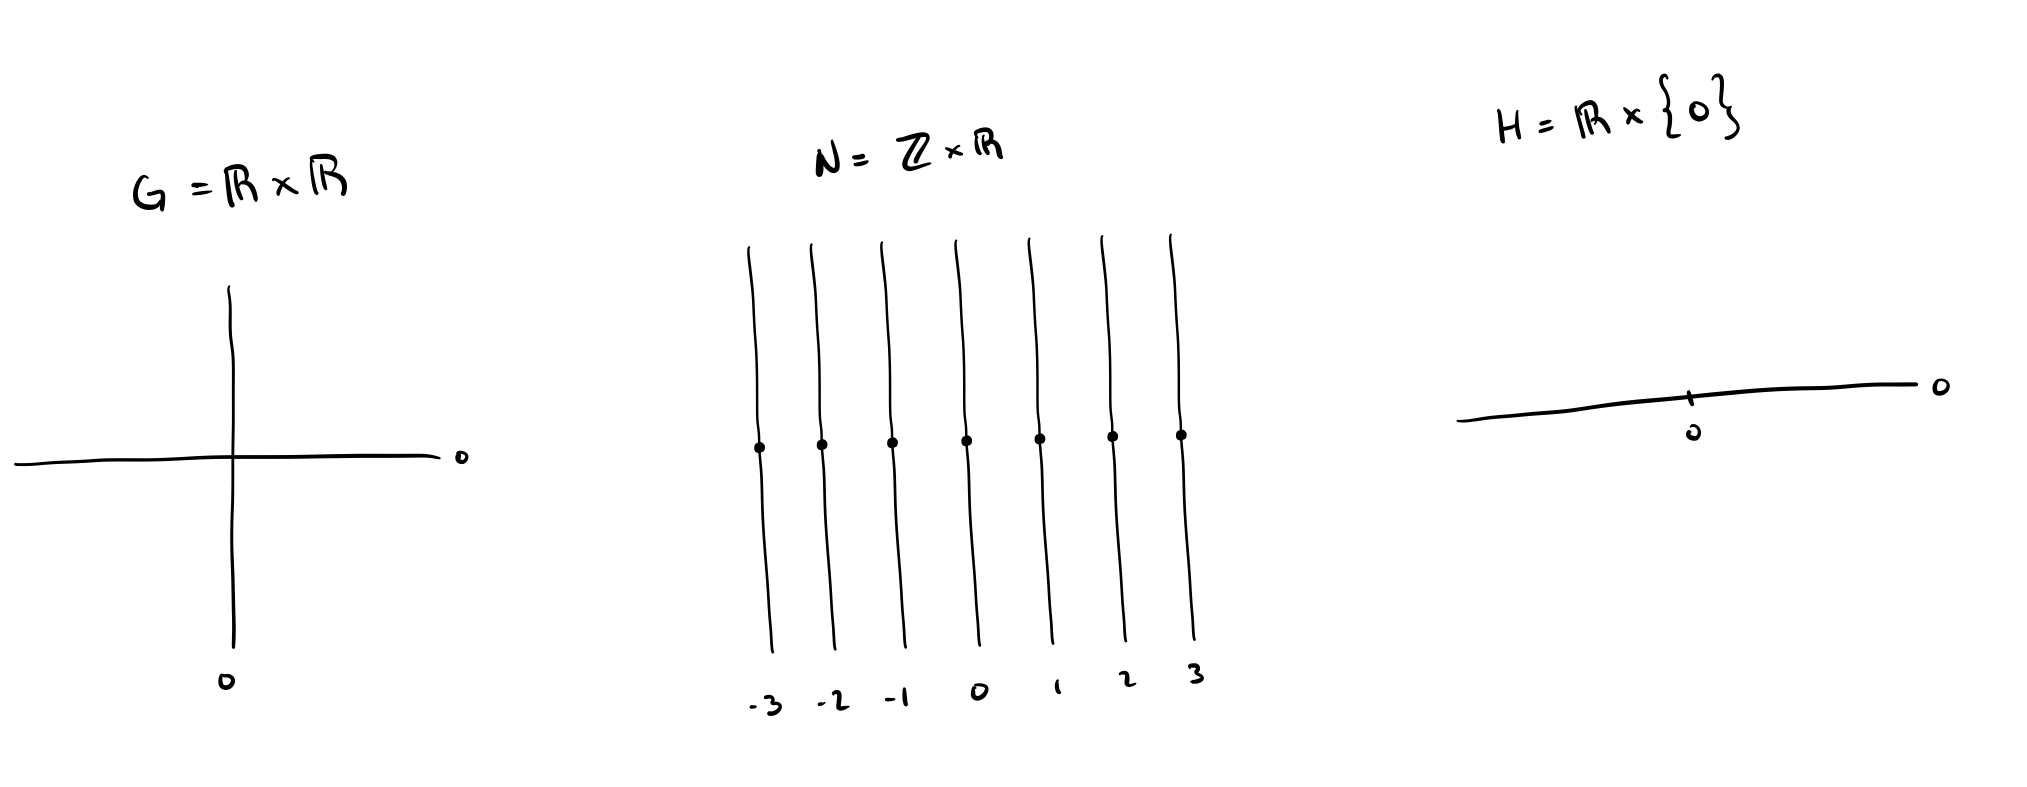
\includegraphics[width=0.75\textwidth]{images/2isothminit}
            \label{fig:2isothminit}
        \end{figure}
        \begin{figure}[h]
            \centering
            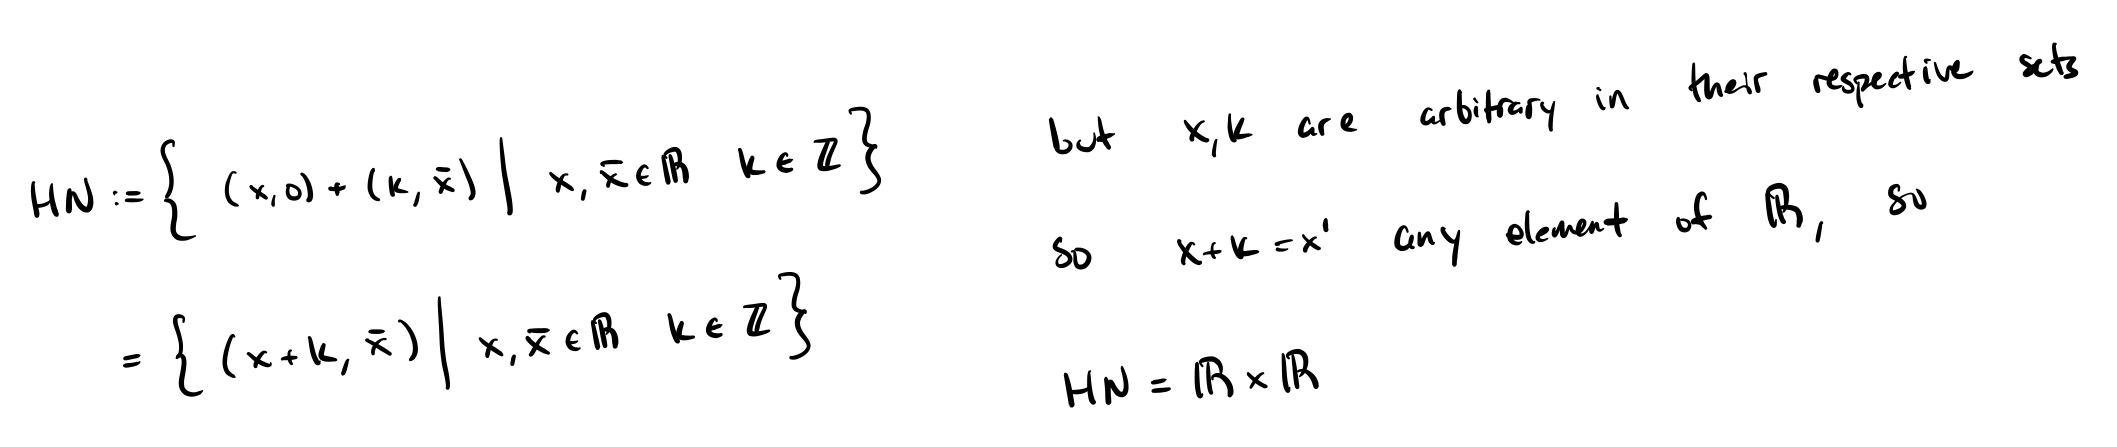
\includegraphics[width=0.75\textwidth]{images/HN}
            \label{fig:HN}
        \end{figure}
        \begin{figure}[h]
            \centering
            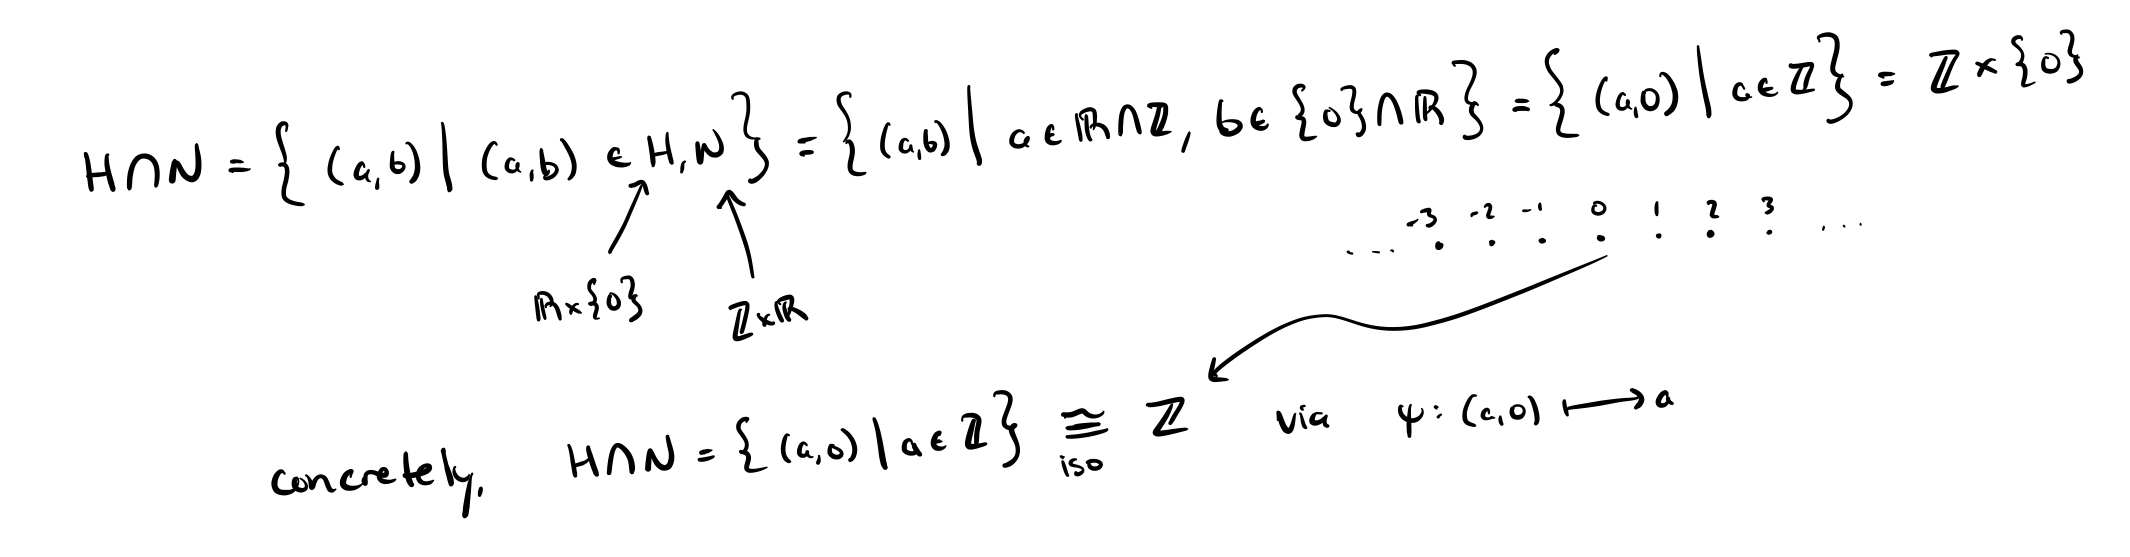
\includegraphics[width=0.75\textwidth]{images/HandN}
            \label{fig:HandN}
        \end{figure}
        \begin{figure}[h]
            \centering
            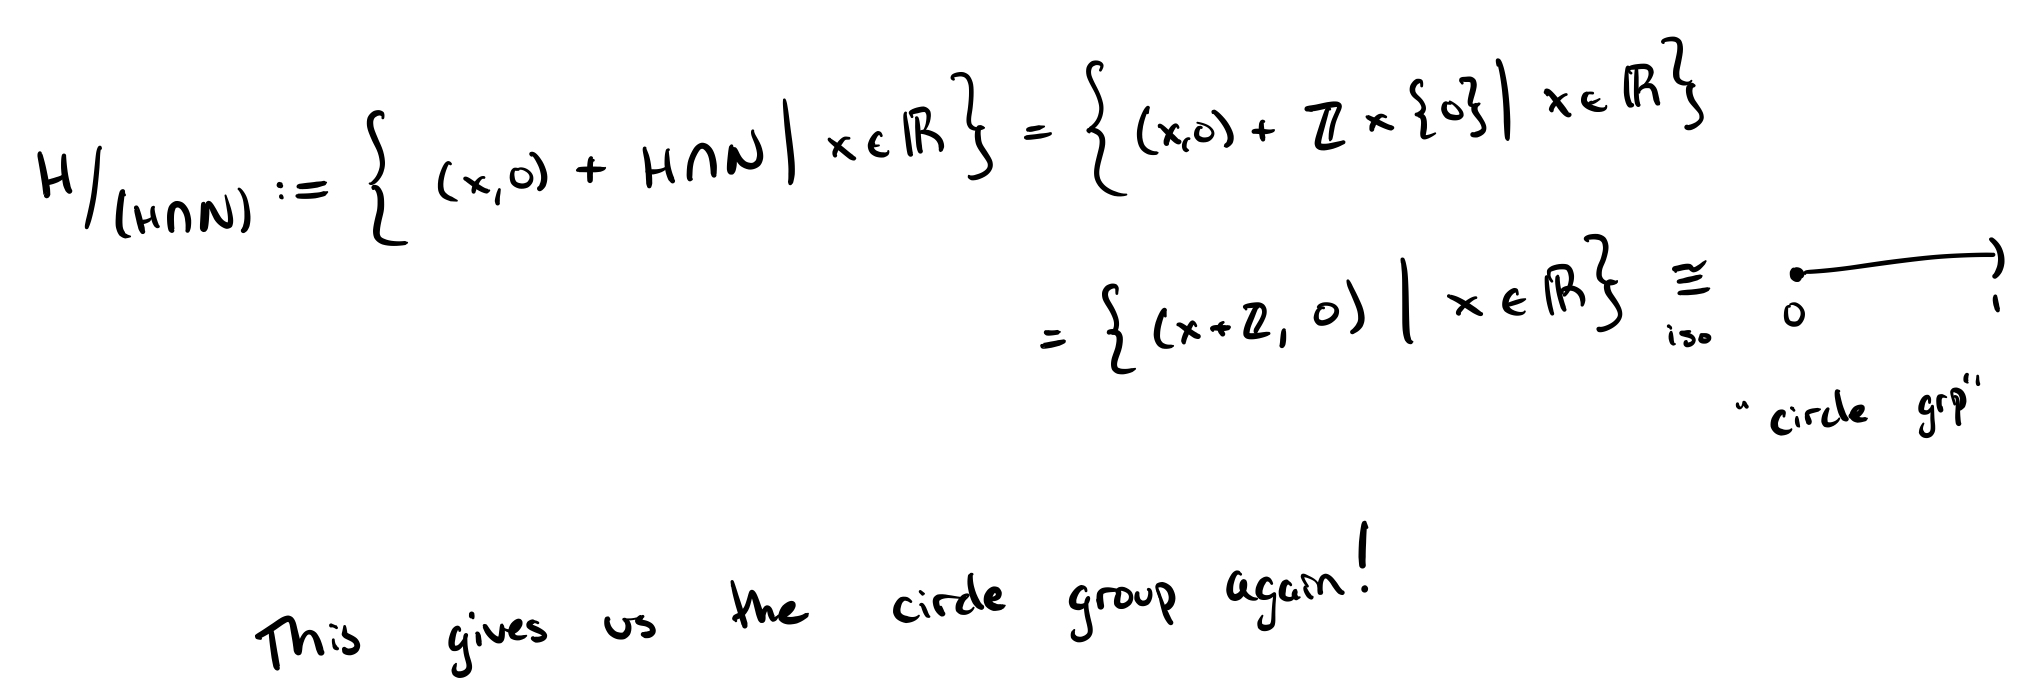
\includegraphics[width=0.75\textwidth]{images/HmodHandN}
            \label{fig:HmodHandN}
        \end{figure}
        \begin{figure}[h]
            \centering
            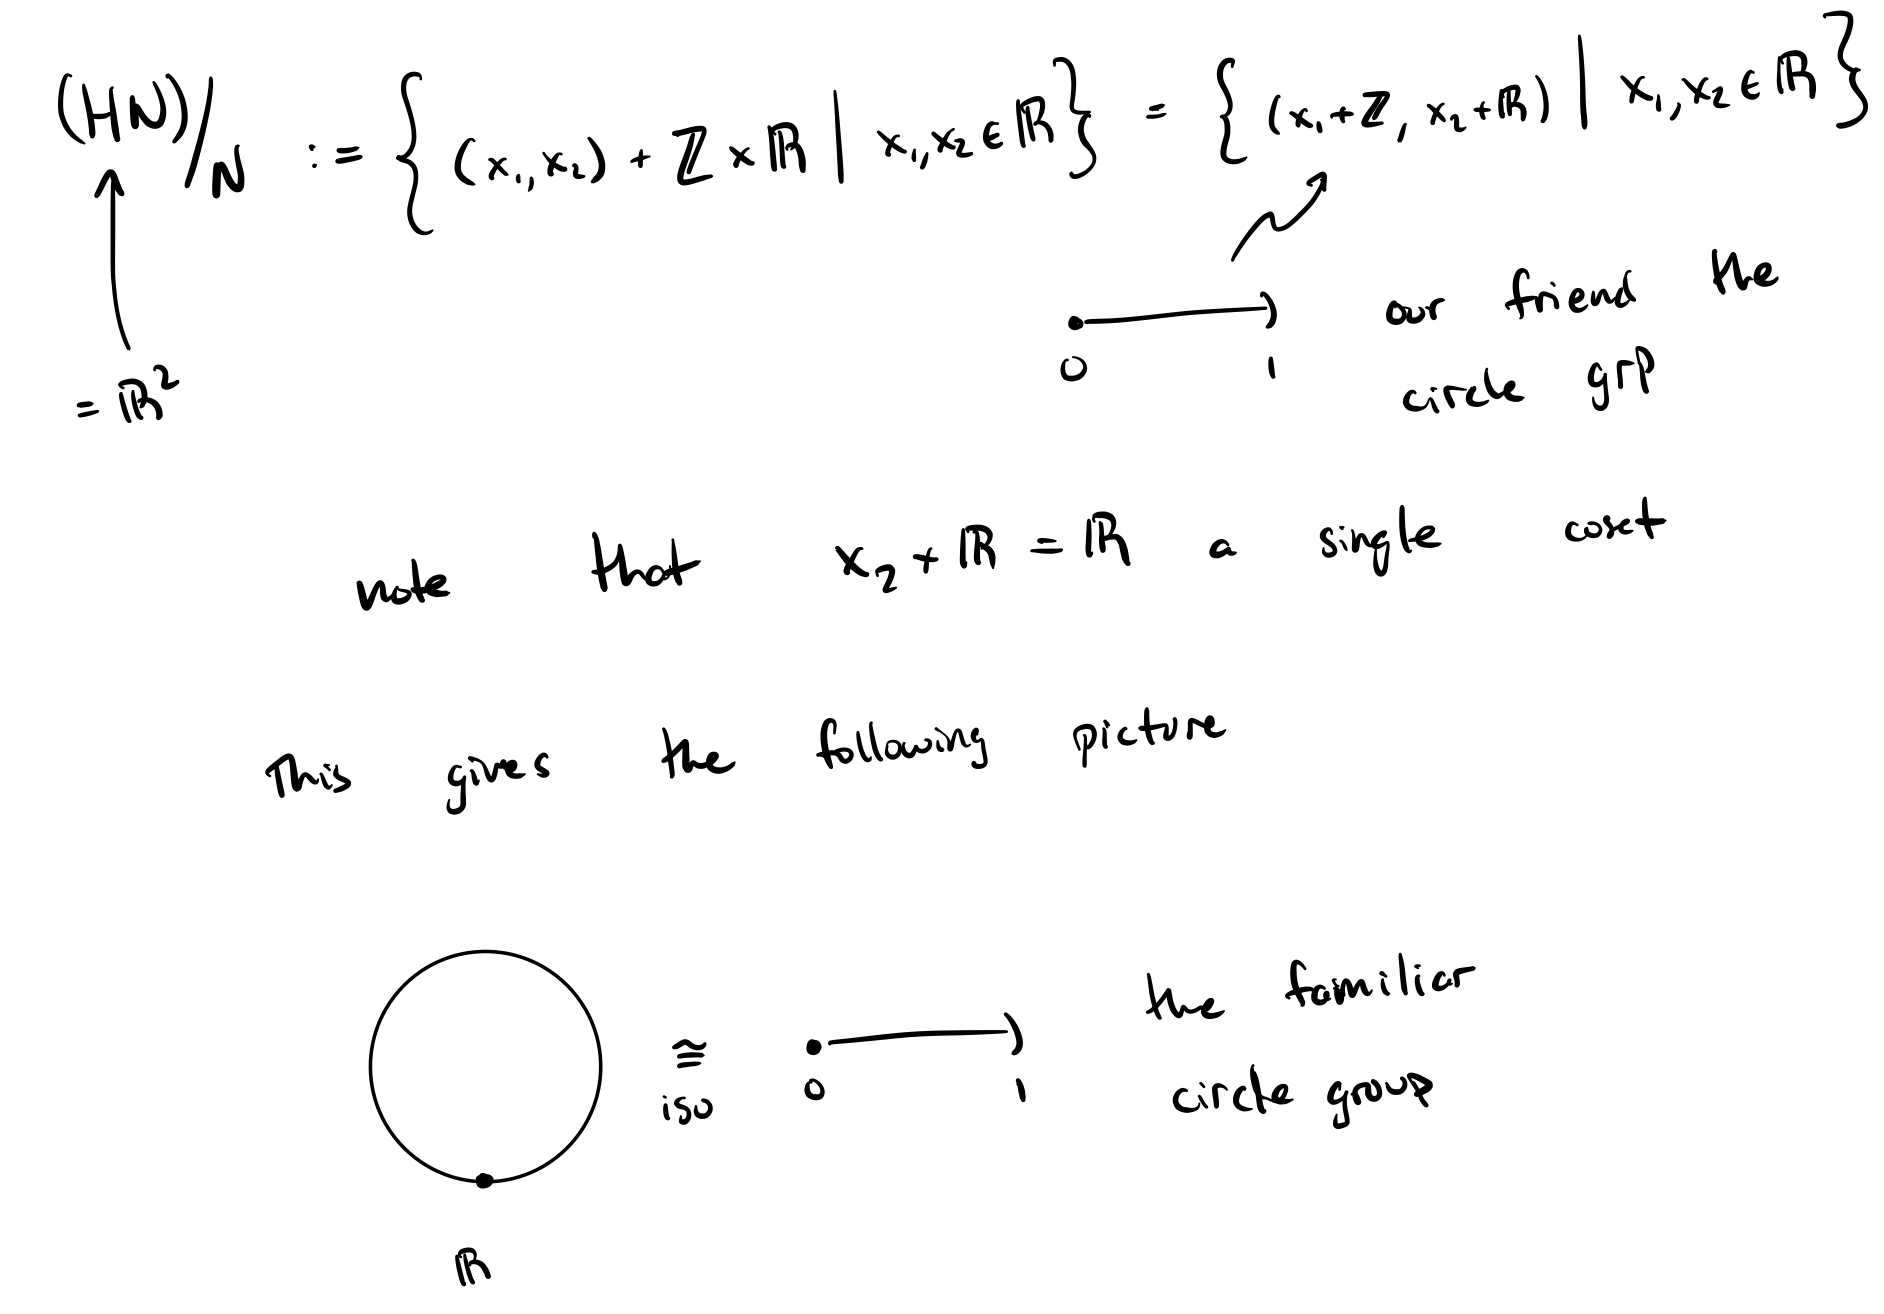
\includegraphics[width=0.75\textwidth]{images/HNmodN}
            \label{fig:HNmodN}
        \end{figure}
        \newpage
        Thus we have depicted the groups!
    }

% hw problem 4 -----------------------------------------------------------------

\begin{exercise}{96}{5}
    \problem{
        Let $G$ be a finite group, $N_1, N_2, ..., N_k$ normal subgroups of $G$ such that $G = N_1 N_2 \cdots N_k$ and $|G| = |N_1| |N_2| \cdots |N_k|$.
        Prove that $G$ is the direct product of $N_1, N_2, \ldots, N_k$.
    }
    \proof{
        This one threw me for a loop, I could not come up with a rigorous proof of the statement.
        Here is what I got.
        $G$ is the direct product of $N_1, N_2, \ldots N_k$ if and only if $N_1 \times N_2 \times \cdots \times N_k$ is isomorphic to $G$.
        Consider the function $\psi: N_1 \times N_2 \times \cdots \times N_k \to G$ defined by taking $(n_1, n_2, \ldots, n_k)$ to $n_1 n_2 \cdots n_k$.
        Since $G = N_1 N_2 \cdots N_k$ we know $\psi$ to be a surjection.
        Furthermore, since $|G| = |N_1| |N_2| \cdots |N_k| = | N_1 \times N_2 \times \cdots \times N_k |$ and each cardinality is finite, we can deduce that $\psi$ is also an injection. \parspace
        It only remains to show that $\psi$ is a homomorphism.
        That is, we must show that
        $$\psi ( (n_1, n_2, \ldots, n_k)) \psi ( (\bar n_1, \bar n_2, \ldots, \bar n_k)) = \psi ( (n_1, \ldots, n_k) ( \bar n_1, \ldots, \bar n_k) ) $$
        Cetainly the LHS is $n_1 \cdots n_k \bar n_1 \cdots \bar n_k$ and the RHS is $\psi ( n_1 \bar n_1, \ldots, n_k \bar n_k) = n_1 \bar n_1 \cdots n_k \bar n_k$.
        However, I could not not figure out a way to show that the RHS equals the LHS.
    }
\end{exercise}

% hw problem 5 -----------------------------------------------------------------

\begin{exercise}{96}{6}
    \problem{
        Let $G$ be a group, $N_1, N_2, \ldots, N_k$ normal subgroups of $G$ such that: \\
        \indent (1) $G = N_1 N_2 \cdots N_k$ \\
        \indent (2) For each $i$, $N_i \cap (N_1 N_2 \cdots N_{i-1} N_{i+1} \cdots N_k) = (e)$ \\
        Prove that $G$ is the direct product of $N_1, N_2, \ldots, N_k$
    }
    \proof{
        We begin with a lemma that is a consequence of property (2).
        Given a fixed $N_i$, let $H_i$ be the product of any selection of $\bar N_i = N_1, ..., N_{i-1}, N_{i+1}, ... , N_k$.
        We claim that $N_i \cap H_i = (e)$.
        Here is the proof.
        Certainly $e \in H_i$ and $e \in N_i$ so $e \in N_i \cap H_i$.
        From property (2), we know that $N$ intersect all the other normal subgroups $N_j$ is $(e)$.
        Further, we know $H_i$ must be a subset of $N_1, ..., N_{i-1}, N_{i+1}, ... , N_k$ for every element of $H_i$ can be written as an element of $\bar N_i $ with $e$ chosen as the element for sets that were not selected for $H_i$.
        Thus we are just constricting one of the sets involved in an intersection (and we certainly keep the elements that are already in the intersection) so $N_i \cap H_i = (e)$. \parspace
        Now let's proceed by induction.
        For a base case, take $K_2 = N_1 N_2$.
        By the lemma just proven, we have $N_1 \cap N_2 = (e)$ and the corollary on page 95 of the textbook tells us that $K_2$ is the internal product of $N_1$ and $N_2$.
        Futhermore, $K_2 \trianglelefteq G$ since $N_1, N_2 \trianglelefteq G$.
        Now supppose for some $j \in \{ 2, 3, ..., k-1 \}$ that $K_j $ is the direct product $K_j = N_1 N_2 \cdots N_j$.
        We will show that $K_{j+1} = N_1 N_2 \cdots N_j N_{j+1} $ is also a direct product.
        The lemma tells us that $K_j \cap N_{j+1} = (e)$ and we can apply the corollary again to say that $K_{j+1}$ is the direct product of $N_1 N_2 \cdots N_j N_{j+1} $. \parspace
        Thus, by induction, every $K_j$ for $j \in \{ 2, 3, ..., k \}$ is the direct product of $N_1 N_2 \cdots N_j$.
        This implies that $G = N_1 N_2 \cdots N_k$ is a direct product as well!
    }
\end{exercise}


\end{document}
